\begin{figure}
    \centering
    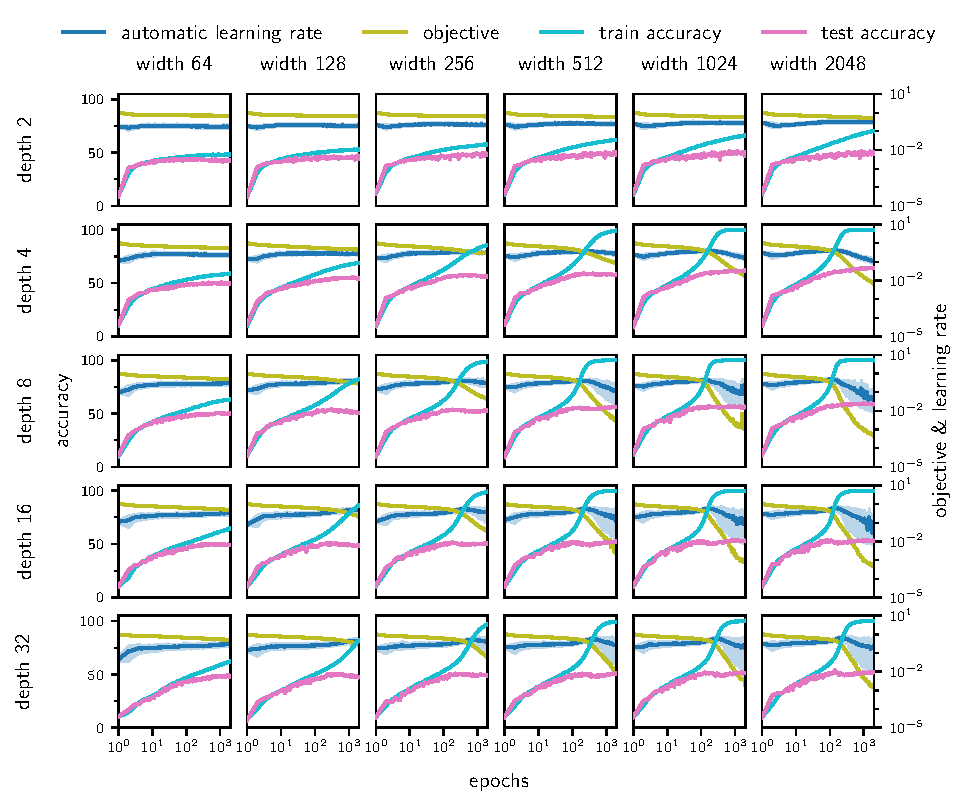
\includegraphics[width=\textwidth]{figures/pdf/plots3_0}
    \caption{\captiontitle{Benchmarking automatic gradient descent on networks of varying width and depth.} We trained fully-connected networks on CIFAR-10 with square loss and a mini-batch size of 128. The depth ranged from $2$ to $32$, and the width from $64$ to $2048$, in powers of two. In terms of training performance, wider was always better, while depth 8 and depth 16 were superior to depth 32. In terms of test accuracy, the best performance was achieved at depth 4 and width 2048: 63.7\%. The worst test performance was achieved by the smallest network of depth 2 and width 64: 42.55\%.
    Larger networks display two broadly distinct phases of training: the automatic learning rate increases slowly while the objective decreases slowly, followed by a rapid decrease in the automatic learning rate and objective. This second phase typically coincides with reaching 100\% train accuracy. See \cref{fig:2} for a comparison between Adam, SGD and AGD for the 256-width 8-layer FCN.} \label{fig:3}
\end{figure}